\section{Multi-player flowchart and explanation~\ref{fig:multiplayer}}

\begin{figure}
    \centering 
    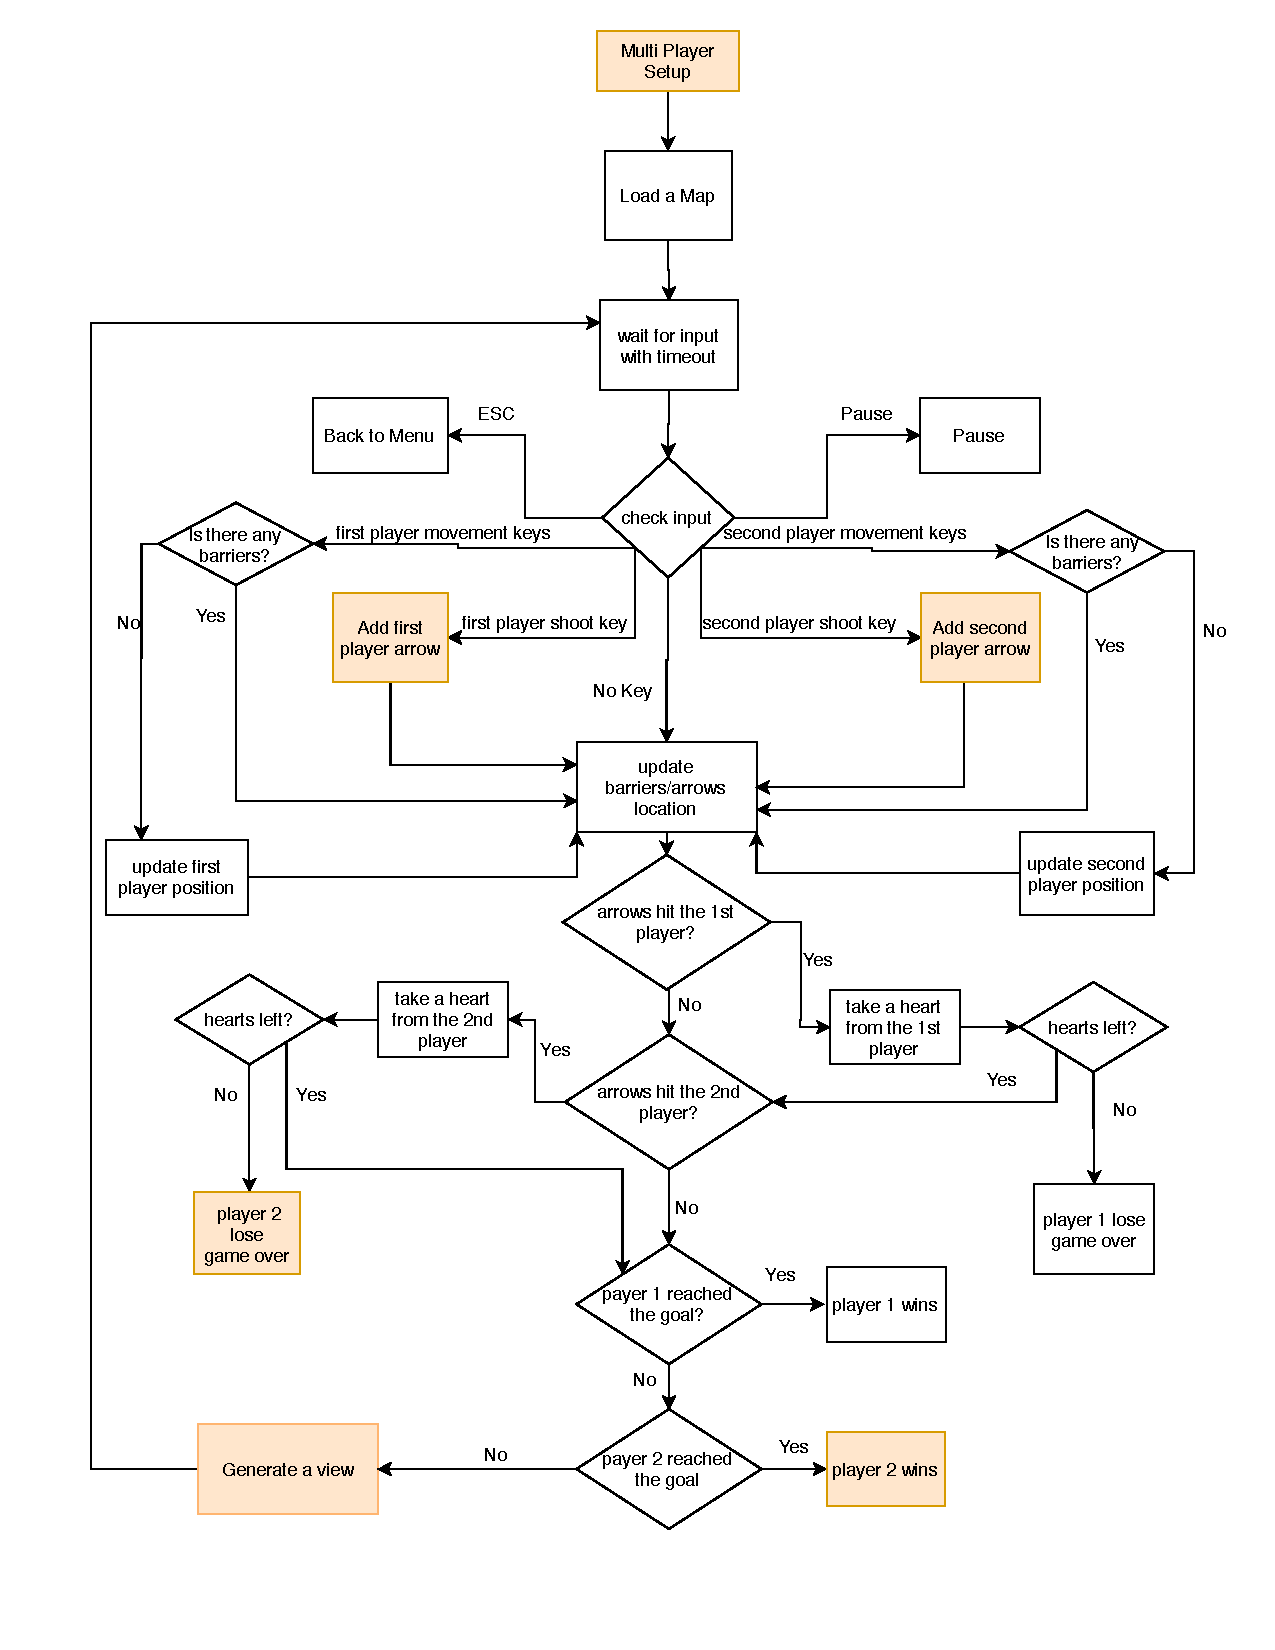
\includegraphics[width=0.9\columnwidth]{multiplayer.pdf}
    \caption{Multi-player block flowchart. Blocks which are in \textcolor{orange}{orange} will be implemented for the second release. Some functions and blocks are used in both single player and multi-player mode which are in white color.}
    \label{fig:multiplayer}
\end{figure}

This Flow chart explains all the steps happening on multi-player mode. 
As it is shown in Figure~\ref{fig:multiplayer}, after we select the multi-player option in Menu function, we begin from the load Map step, where we should read the map from a text file. 
Next, we do some setups for multi-player game based on the map. 
In these setups, we define a map with positions of two players, the goal, the barriers and the arrows. 
We should then get input from keyboard. 
We should check if there was any input given for either player. 
If not, we should update the position of barriers/arrows as they are moving objects. 
If either player hits delete/ backspace button, we go back to menu. 
If hits space button, we go to the state of pause game. 
If hits space button again, we should continue the game. 
In both continue and pause state, we go back to get input from keyboard and wait for either player to enter another key. 
Given the movement keys, we update the position of first/second player accordingly. 
Also, by giving the specific shoot keys, we then generate arrows from the position of the shooting player. 
Both players need to run in different directions controlled by movement keys to avoid being shot by moving arrows. 
The process of dealing with barriers, losing hearts and reaching the goal for each player is the same as single player mode. 
By continuing to check the remaining hearts of them during the whole movement, we can know which player loses the game earlier than the other, which is the same way as judging whether the game is over for single player mode. 
As for the win scenario, only if the player alive reaches the final goal. 
If not reaching the win state ever, the program will generate a view afterwards and continue to wait for another key input.

\subsection{Multi-player functions prototypes}

In this section we define the required functions prototypes and its relation to flow chart~\ref{fig:singleplayer}. We define some functions and the rest of the code will be in a main multi-player function. Comments above each function mention the associated block, the release, and assignee. Some functions are in common for both single player and multi-player mode.We did not mention then again as they already described.

\begin{minted}{c}
/**
 * @brief timer
 * @author Pari
 * First Release
 */
Uint32 timer_callback(Uint32, void*);

/**
* @brief generate_view_multi function
* @author Jin
* Release two
* This function is to generate a graphic map using updated information
* @param[in] p_window a SDL window which is passed from the main function.
* @param[in] p_map a defined map which is passed from the main function.
* @return: void
*/
void generate_view_multi(SDL_Window* p_window, map_t* p_map);

/**
 * @brief Generates a bullet
 * @author Mahsa
 * Release two
 * This function generates a bullet in the player's current position
 * and initialize the speed and direction.
 * @param[in] map represent the map structure which has players' position.
 * @param[in] player_num represent the player index: PLAYER_1/PLAYER_2.
 */
void shoot(map_t* map, player_index_t player_num);

/**
 * @brief updates the position of generated bullet
 * @author Mahsa 
 * Release two
 * This function shoot a bullet in a direction in which an oppenent exists.
 * @param [in] map represent the map structure which has bullet's position and direction.
 */
void update_bullet(map_t* map, player_index_t player_num);

/**
 * @brief Checks if a bullet hit a player.
 * @author Mahsa 
 * Release two
 * This function checks if the player is hit by oppent's bullet.
 * @param [in] map represent the map structure which has 
 * player position and bullets' positions.
 * @param [in] player_index  can be PLAYER1 or PLAYER2.
 * @return flag if the player is hit, flag = 1, otherwise flag = 0.
 */
int is_bullet_hit(map_t* map, player_index_t player_index);
\end{minted}